\documentclass[10pt]{beamer}
\usepackage{xeCJK}
\usepackage{graphicx}
\usepackage{booktabs}
\usepackage{listings}
\usepackage{multirow}
\usepackage{mathtools}
\usepackage{ulem}
\usetheme{metropolis}
\begin{document}
\title{水题讨论}
\date{\today}
\author{huhao}
\maketitle
\clearpage
\begin{frame}
	\frametitle{Prologue}

	\onslide<1-> 题目大家可能见过,\sout{见过可以重开一遍。}

	\onslide<2-> 题目不涉及高深算法/数据结构。

	\onslide<3-> 由于题目设计转化、构造等,一眼秒了可以略微给其它同学一些思考时间。

	\onslide<4-> \sout{应该有需要画图的部分,可能需要一位好心人拍下黑板。}
\end{frame}
\clearpage
\begin{frame}
	\frametitle{1.1 AGC040F Two Pieces}

	你有两个棋子,若某时刻棋子位置为:$(a,b)$($a\le b$),那么你可以让它们位置变为:$(b,b),(a+1,b),(a,b+1)$  

	棋子不作区分,问$t$时刻后棋子位置为$(x,y)$的方案  

	两方案不同当且仅当某时刻棋子位置不同  

	$1\le t\le 10^7,0\le x\le y\le t$

	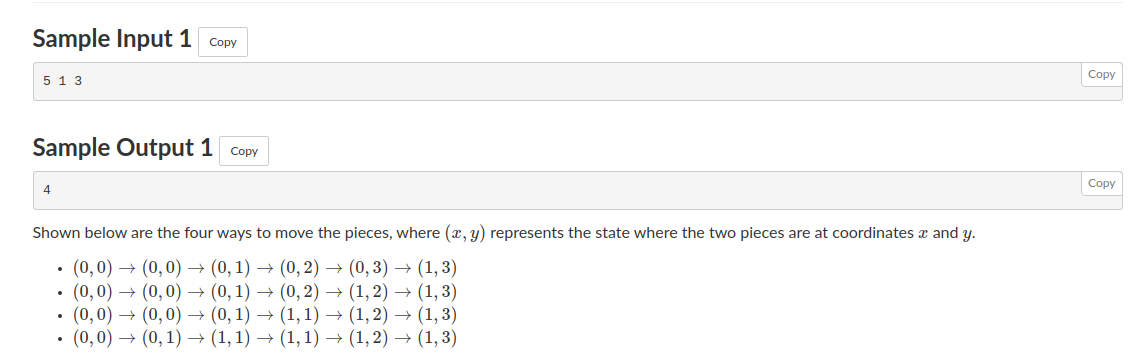
\includegraphics[width=0.9\textwidth]{1.png}

\end{frame}
\clearpage
\begin{frame}
	\frametitle{1.2 AGC040F solution}

	\onslide<1-> 记状态$(a,b)$表示位置$(a,a-b)$,那么每一次可以变为:$(a+1,b+1),(a,b-1),(a,0)$

	\onslide<1-> 为了去重,第二个操作要求$b\ge 2$

	\onslide<2-> 于是我们可以记一个由$\{1,2,3\}$组成的操作序列,表示第$i$次的操作

	\onslide<2-> 那么操作序列长为$t$,且$1$出现$y$次

	\onslide<3-> 于是可以只考虑$b$的值,考虑枚举$3$出现次数$t_0$

	\onslide<4-> 若$t_0=0$,则是一个经典的格路计数题:求由$(0,0)$走到$(t-y,y-x)$,每一次可以走向量$(1,-1)$或$(1,1)$,不经过$y=0,x>0$的方案数

	\onslide<5-> 考虑推广,不考虑$3$的话会是一个到$(t,y-(t-y-t_0))$的路径,只要在纵坐标为$y-(t-y-t_0)-(y-x)$时执行一次$3$操作即可

	\onslide<6-> 另外如果一个位置可以插入$3$当且仅当后面的纵坐标都比它大,所以转化为:一共$y-(t-y-t_0)-(y-x)+1$个位置,且最后一个必须放,前面的可放可不放,问方案数

\end{frame}
\clearpage
\begin{frame}
	\frametitle{2.1 IOI2018 机械娃娃}

	这\sout{不}是一道交互题

	有$3$种机械娃娃,分别为\textbf{起点,触发器,开关}。\textbf{起点}有$1$个(编号为$0$),\textbf{触发器}有$m$个(编号$1\sim m$),\textbf{开关}有$s$个(编号$-s\sim -1$),$1,m$为题目给定的,$s$为你给定的。

	运行过程可以理解为一个\textbf{球}在机械娃娃里运动,一开始\textbf{球}在\textbf{起点},\textbf{开关}有$2$个出口(编号$X,Y$),其它的有$1$个出口,每个出口都通向另一个娃娃。

	当球在非\textbf{开关}的娃娃处时,球沿出口运动到下一娃娃;球在\textbf{开关}处时,若球是奇数次来到这个娃娃处,球沿$X$运动到下一娃娃,否则沿$Y$。

	当球经过\textbf{触发器}时,会记录下此\textbf{触发器}编号。
\end{frame}
\clearpage
\begin{frame}
	\frametitle{2.1 IOI2018 机械娃娃}
	给定$m$,并给定一个长度为$n$的数组$A$,你需要设计一个合法的管路(即确定出口编号),满足:

	球会再次经过\textbf{起点},且再次经过时:

	\begin{itemize}
		\item 所有\textbf{开关}经过偶数次,且经过的总次数不大于$2\times 10^7$。
		\item 经过\textbf{触发器}$n$次,且记录下的恰好为数组$A$
	\end{itemize}

	$n\le 2\times 10^5$,要求$s\le n+\lceil\log_2n\rceil$

	\onslide<2->Hint: 想想$n=3/n=7$
\end{frame}
\clearpage
\begin{frame}
	\frametitle{2.2 IOI2018 机械娃娃 Hint}

	\onslide<1-> 显然的思路:新增一个“起点”,经过起点第$i(i\le n)$次后会过$A_i$并再次回到“起点”,经过第$n+1$次后回到起点

	\onslide<2-> 由此,可以手玩出$n=4,m=4,A\mathrm{~is~unique}$的情况
	
	\onslide<3-> 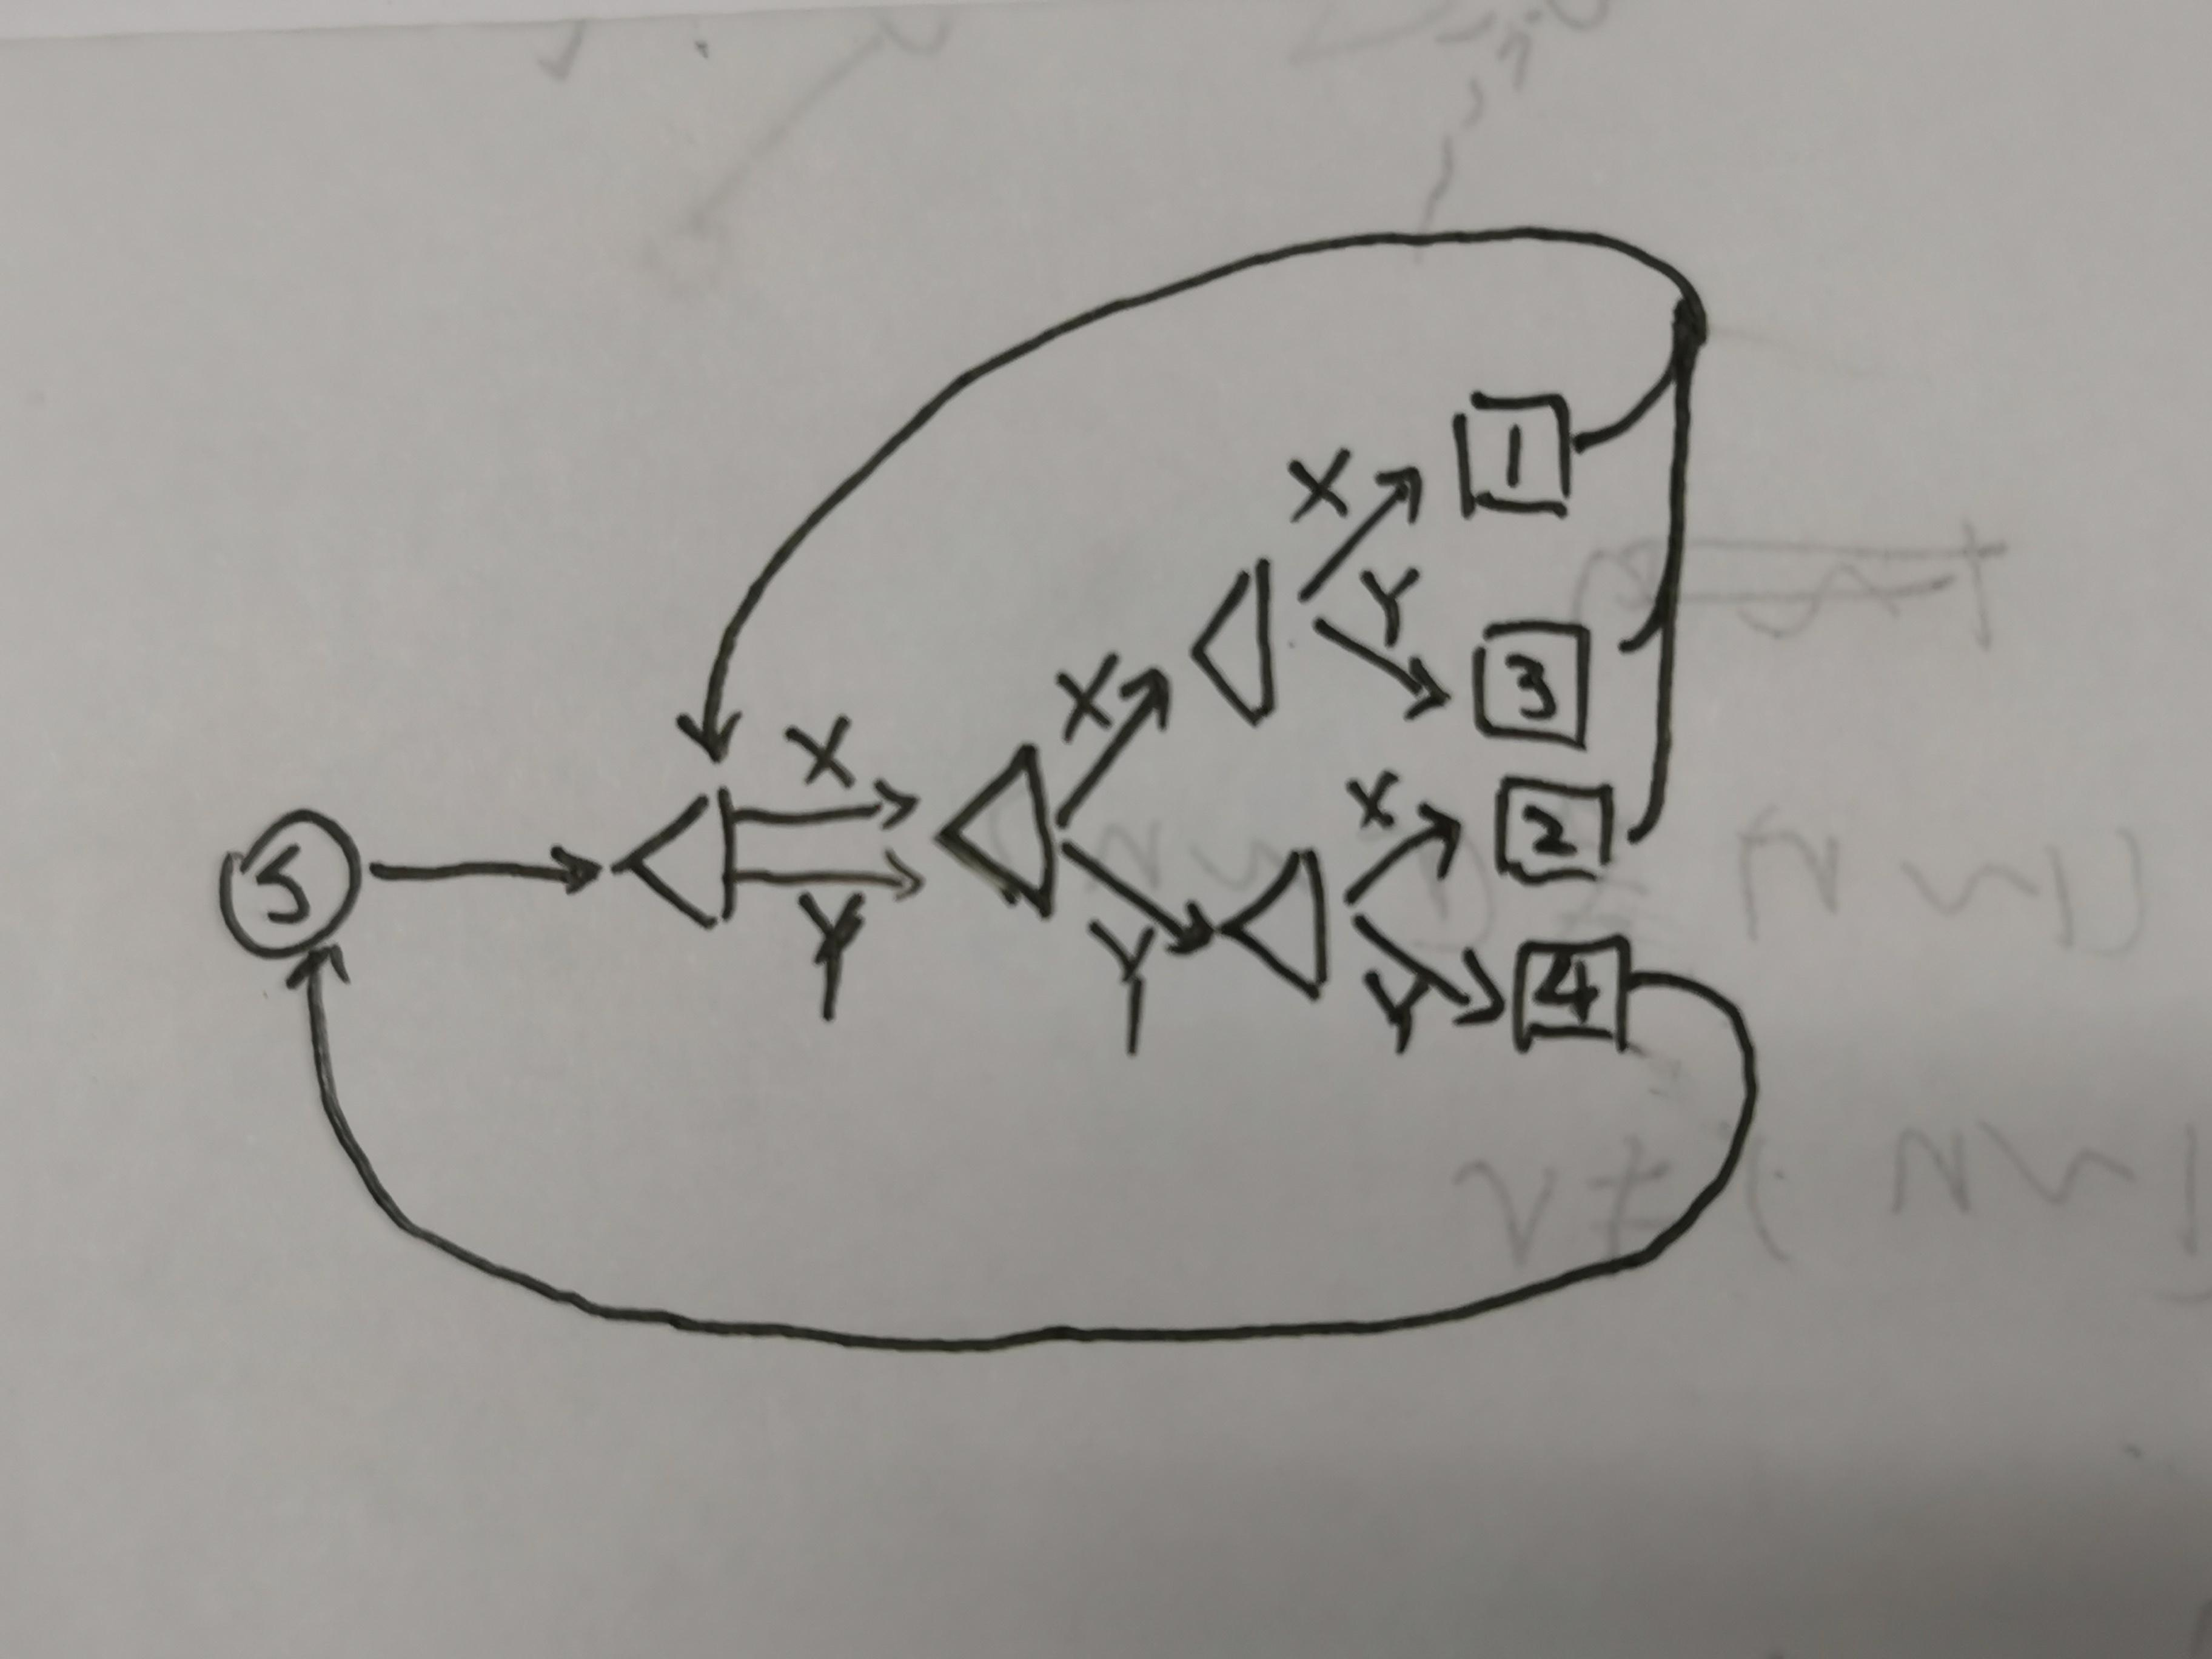
\includegraphics[width=0.7\textwidth]{2.jpg}

\end{frame}
\clearpage
\begin{frame}
	\frametitle{2.3 IOI2018 机械娃娃 solution}

	\onslide<1->于是对于$n=2^k-1$的情况,可以建一颗线段树,叶子就是每一个触发器,起点可以视为第$2^k$个叶子。

	\onslide<2->对于其它情况,可以视为连了一个空叶子(即直接连向“起点”),这样可以用$s=4n$解出此题。

	\onslide<3->如果一个开关两条边都连向“起点”,可以删去这个点,又有触发器只与相对顺序有关,只有代表开关的叶子固定了位置。
	
	\onslide<4->于是可以尽可能地用靠近这个叶子的点(也就是最后面的$n+1$个点,其中代表开关的叶子在倒数第$1$号点),可以证明,这只用到$n+\lceil\log_2n\rceil$的开关

\end{frame}
\clearpage
\begin{frame}
	\frametitle{Epilogue}

	\begin{center}
		\Huge Thanks for listening!
	\end{center}

\end{frame}
\end{document}